\section{Design}
Snake-spillet er lavet efter et Model-View-Control design (MVC). Styringen, spil logikken og den visuelle repræsentation holdes adskilt i tre dele. Med dette bygges et meget modulært program. Spil logikken er Model, styringen er Control og den visuelle repræsentation er View. Disse tre dele skal kode mæssigt holdes adskilt. Spil logikken må ikke kende til styringen eller repræsentationen. Repræsentation må ikke kende til styringen. Styringen må godt kende til spil logikken og repræsentationen, se \figref{mvc} for en illustration.

\begin{figure}[h]
	\centering
   	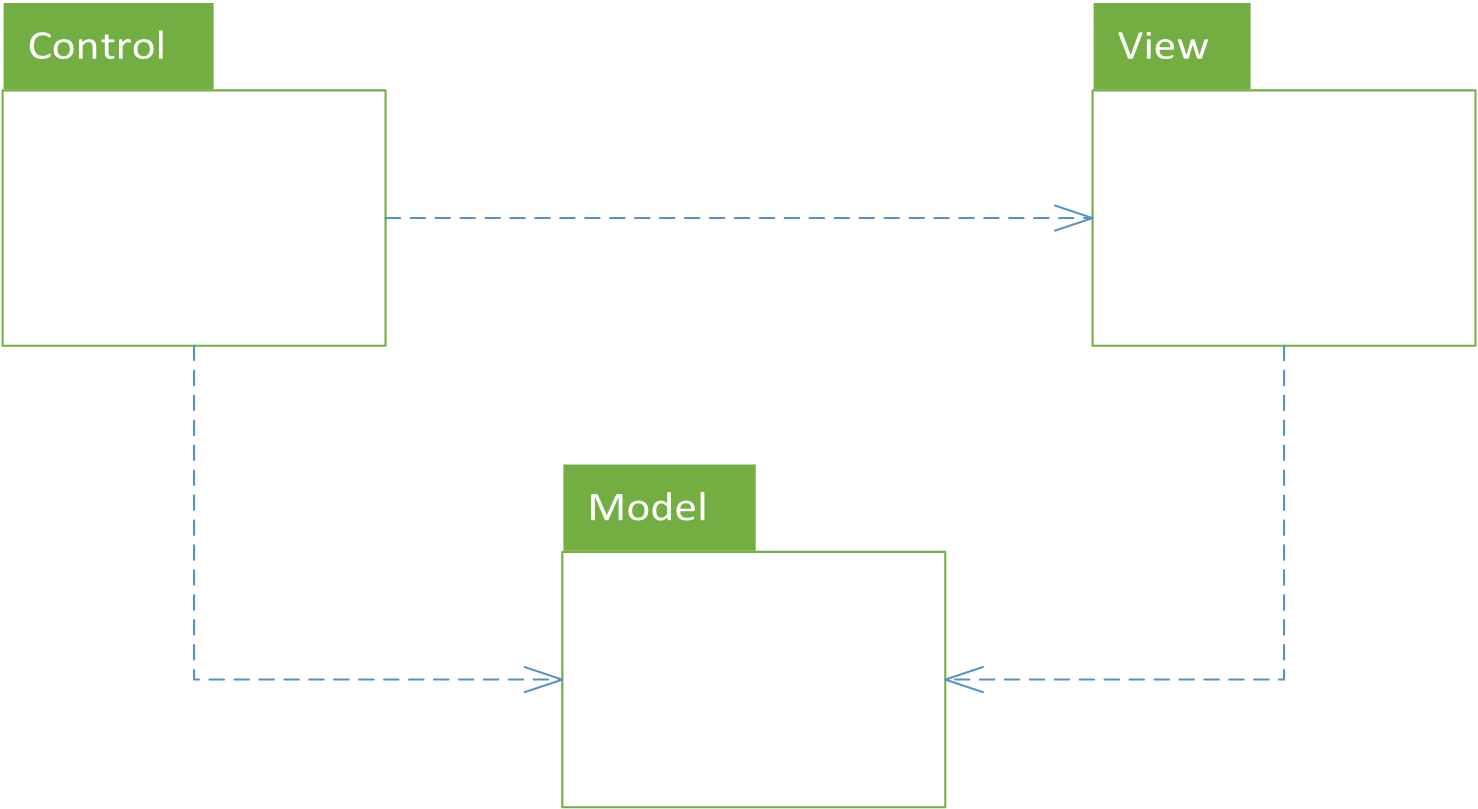
\includegraphics[width=0.7\textwidth]{grundlaeggende/mvc.png}
	\hspace{0.1\textwidth}
	\caption{\figlab{mvc}Oversigt over Model-View-Control design.}
\end{figure}

Brugeren interagere med den del der er dedikeret til styring (Control). Control manipulerer spil logikken (Model) og spillet visualiseres i View-koden. Funktioner, der påvirker programmets tilstand, holdes i Model-koden. Control modtager input fra brugeren og kalder relevante metode i View og Model. View må ikke ændre på spillets tilstand, det skal kun vise hvad der er i Model. 

Man kan tænke på det sådan at View observere Model og viser hvad den ser til brugeren. Control kommunikere med brugeren og sender relevant kommunikation videre til View eller Model.

Simpel Snake er designet, så spillets logik ligger i \textit{Game} klassen i Model-pakken. \textit{Game} indeholder relevante klasser, som for eksempel \textit{Food} og \textit{Snake}. Se \figref{modelsimple}. Vi har valgt at lave en enumerations klasse \textit{Direction}. Den forsimpler kommunikationen til \textit{Game}. Det er nemmere at tilkoble kommandoer og statements til hver retning, hvis der eksplicit er en \textit{Direction} klasse som begrænser retnings mulighederne. Vi har valgt at gøre \textit{Game} til en \textit{Observable}. Med dette kan vores View klasser observere spil logikken og opdatere det som brugeren ser, så snart spillets tilstand ændrer sig. \textit{Snake} klassen afhænger af \textit{Game} klassen fordi at \textit{move} metoden i \textit{Snake} er nød til at signalere til \textit{Game} at slangen har bevæget sig. Dette gør den ved at kalde \textit{snakeHasMoved}.

\begin{figure}
	\centering
   	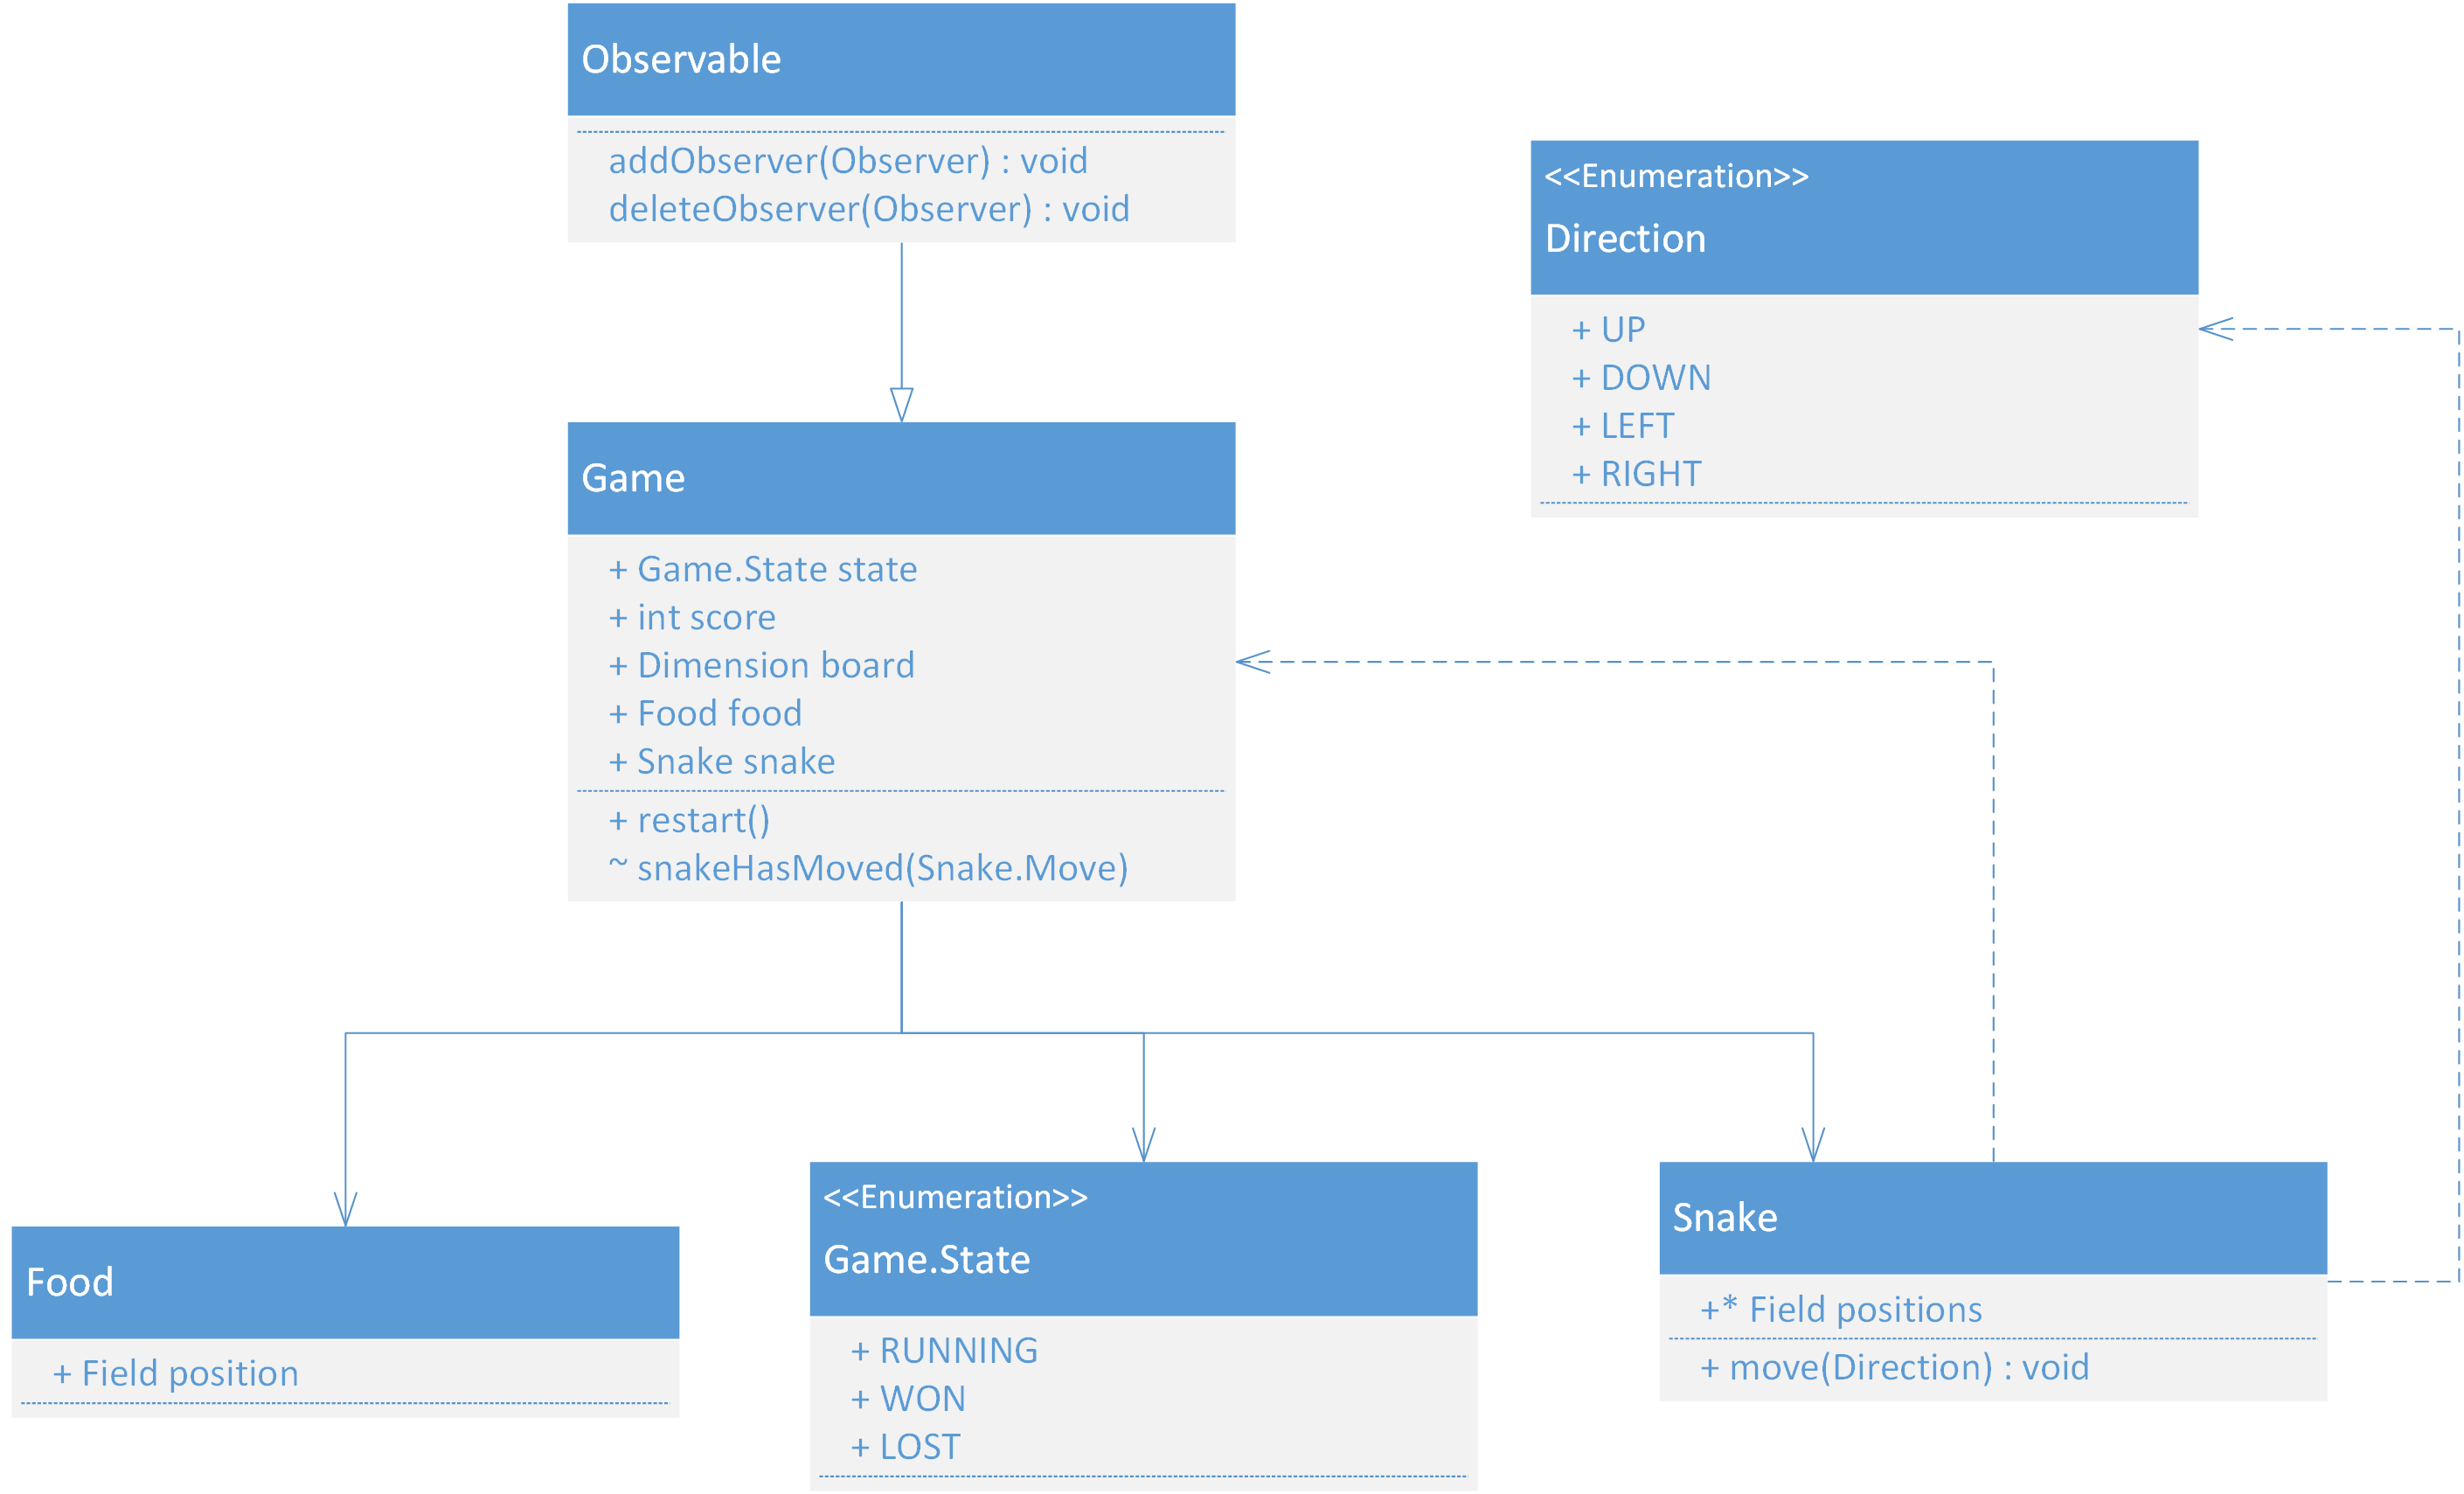
\includegraphics[width=1.0\textwidth]{grundlaeggende/model.png}
	\hspace{0.1\textwidth}
	\caption{\figlab{modelsimple}Oversigt over vores Model design.}
\end{figure}

I \textit{View} klassen har vi vores vindue som brugeren ser spillet igennem. Det har en \textit{BoardPanel} klasse som viser den nuværende spil tilstand. \textit{BoardPanel} nedarver fra \textit{Observer} og opdatere panelet hver gang spillets tilstand ændres. Når dette sker tegnes den nuværende bane, slange og mad som er i \textit{Game} objektet. For eksempel bruges \textit{getSnake()}, til at bestemme slangens position. Scoren holdes i \textit{Game} objektet. \textit{ScorePanel} ligger som et panel over \textit{BoardPanel} i vinduet. Den observere \textit{Game} og opdatere sig selv når scoren ændre sig. Se \figref{viewsimple}.

\begin{figure}
	\centering
   	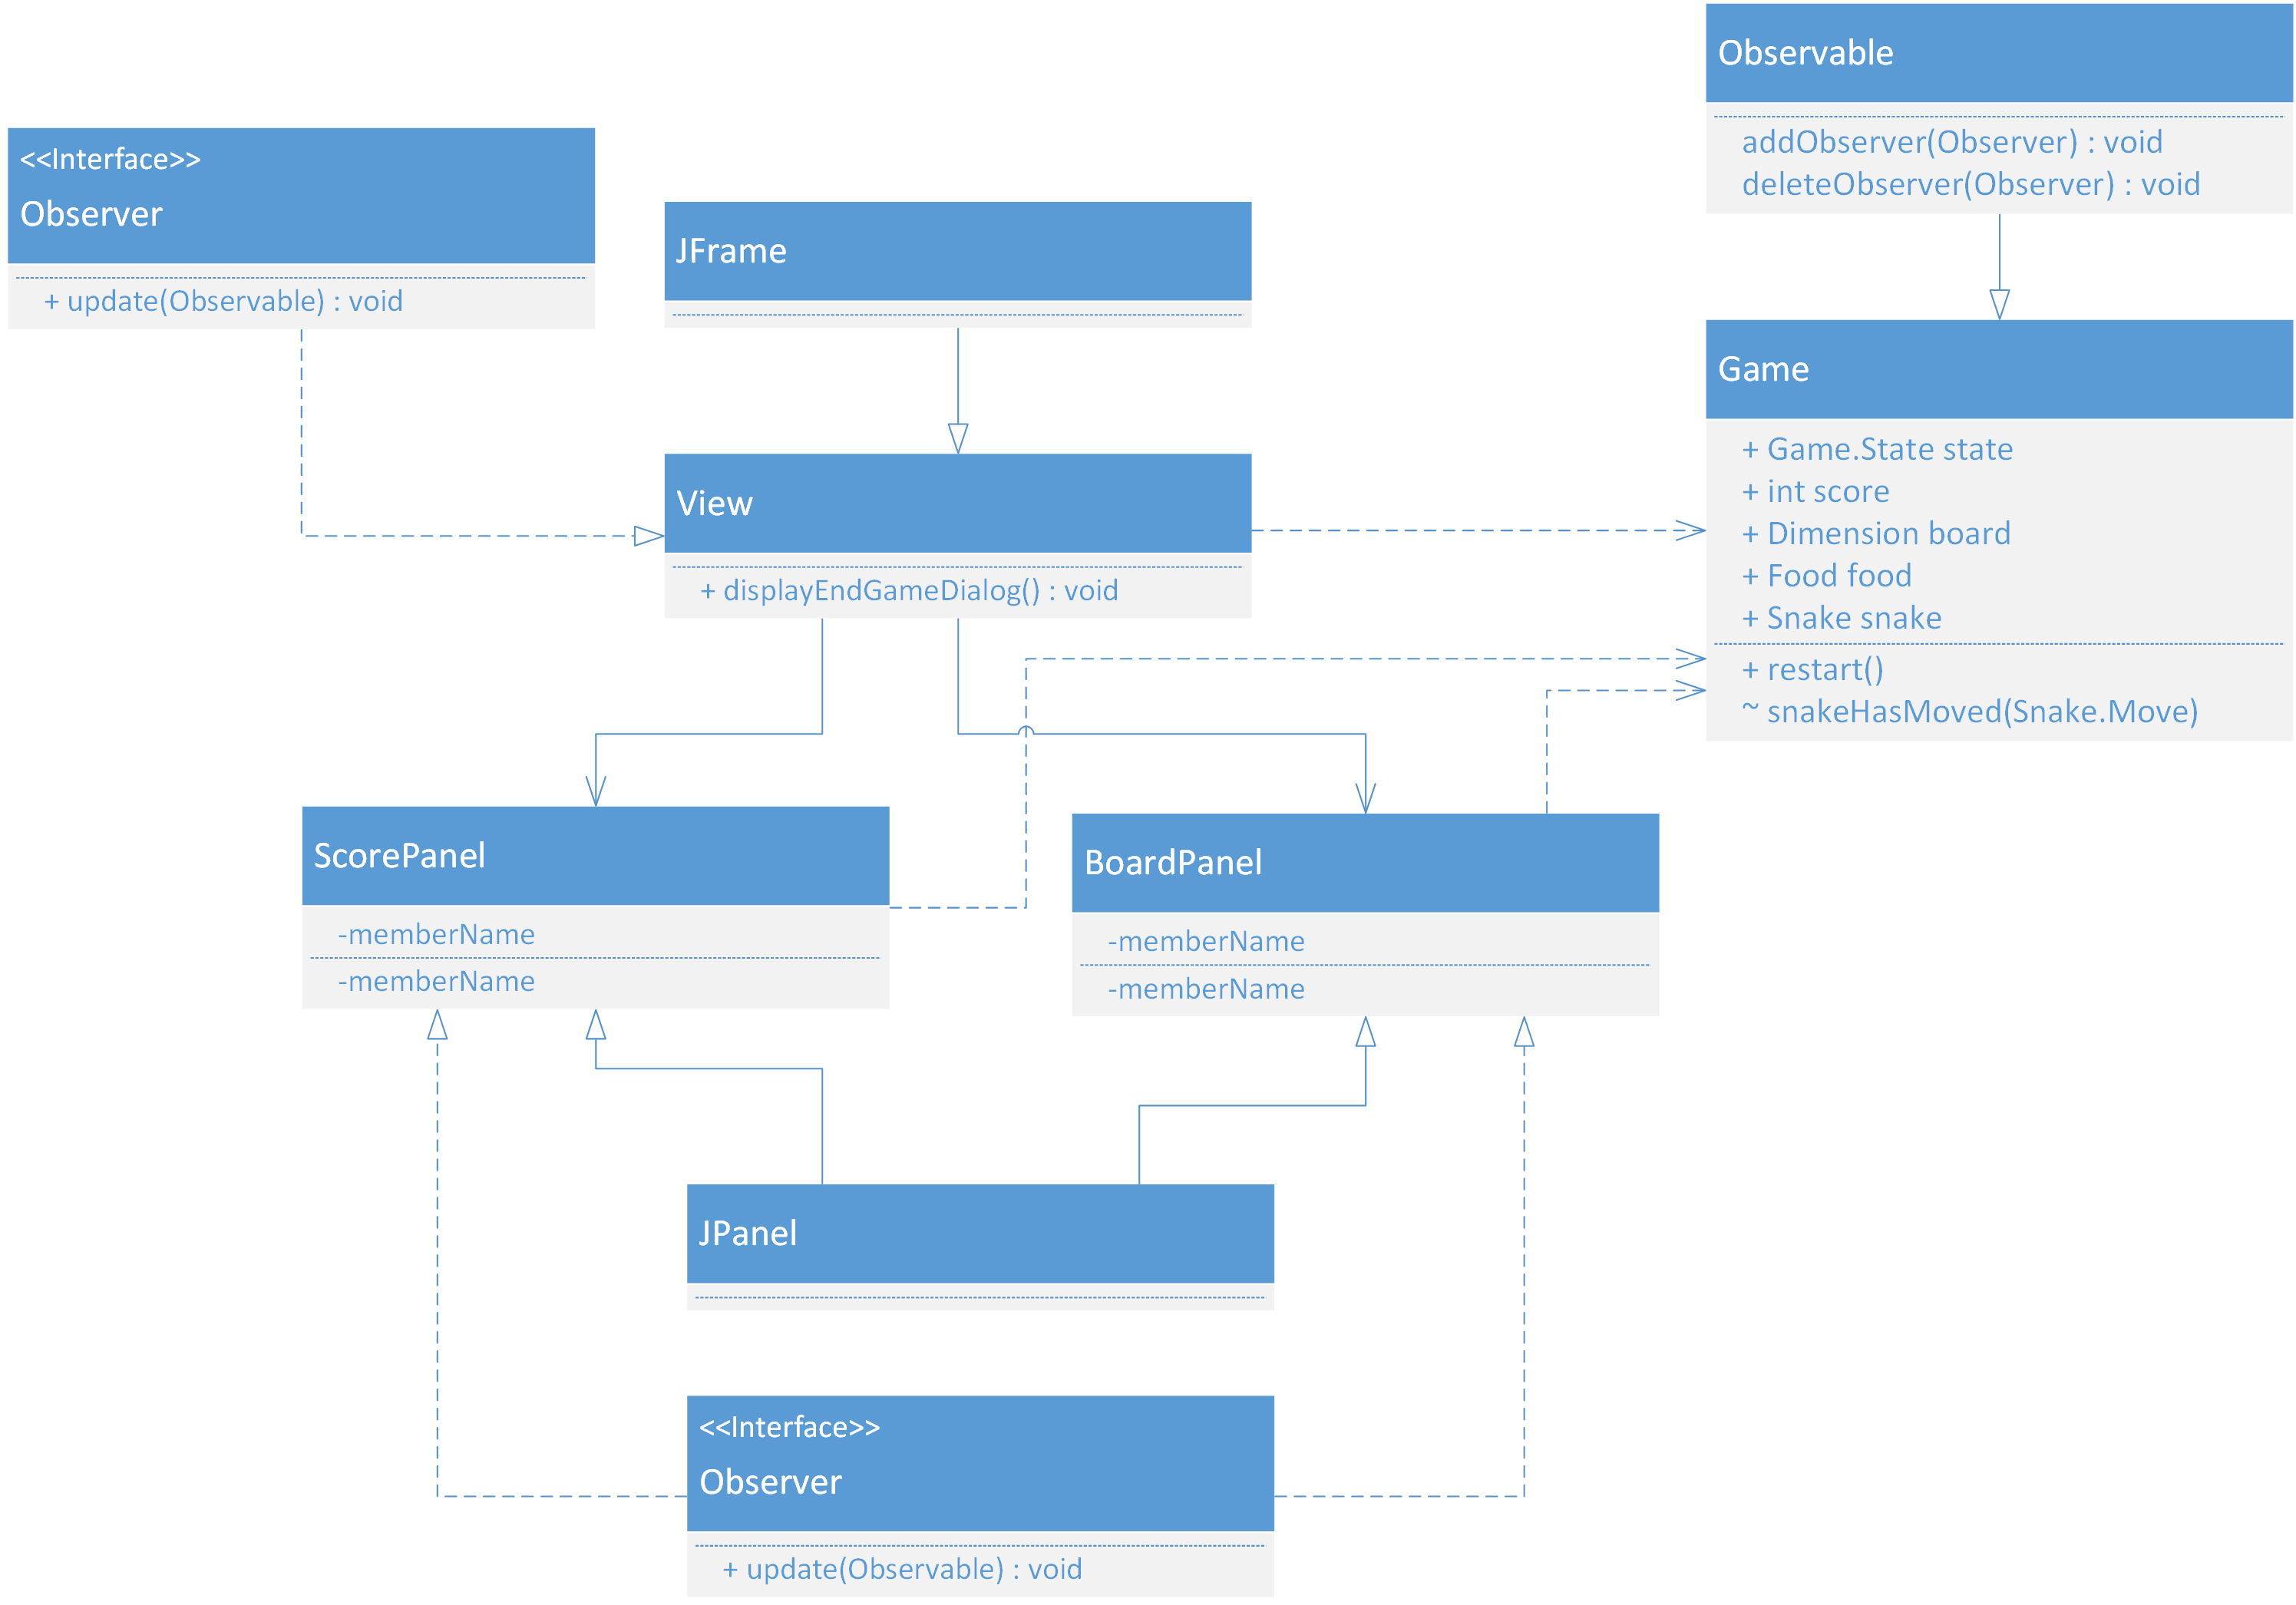
\includegraphics[width=1.0\textwidth]{grundlaeggende/view.png}
	\hspace{0.1\textwidth}
	\caption{\figlab{viewsimple}Oversigt over vores View design.}
\end{figure}

\textit{Control} klassen kalder relevante \textit{Game} og \textit{Snake} metoder når brugeren trykker på dens keyboard. Den bestemmer hvornår og hvorhen slangen skal bevæge sig. \textit{Control}-klassen nedarver fra en KeyListener. Se \figref{controlsimple}.

\begin{figure}
	\centering
   	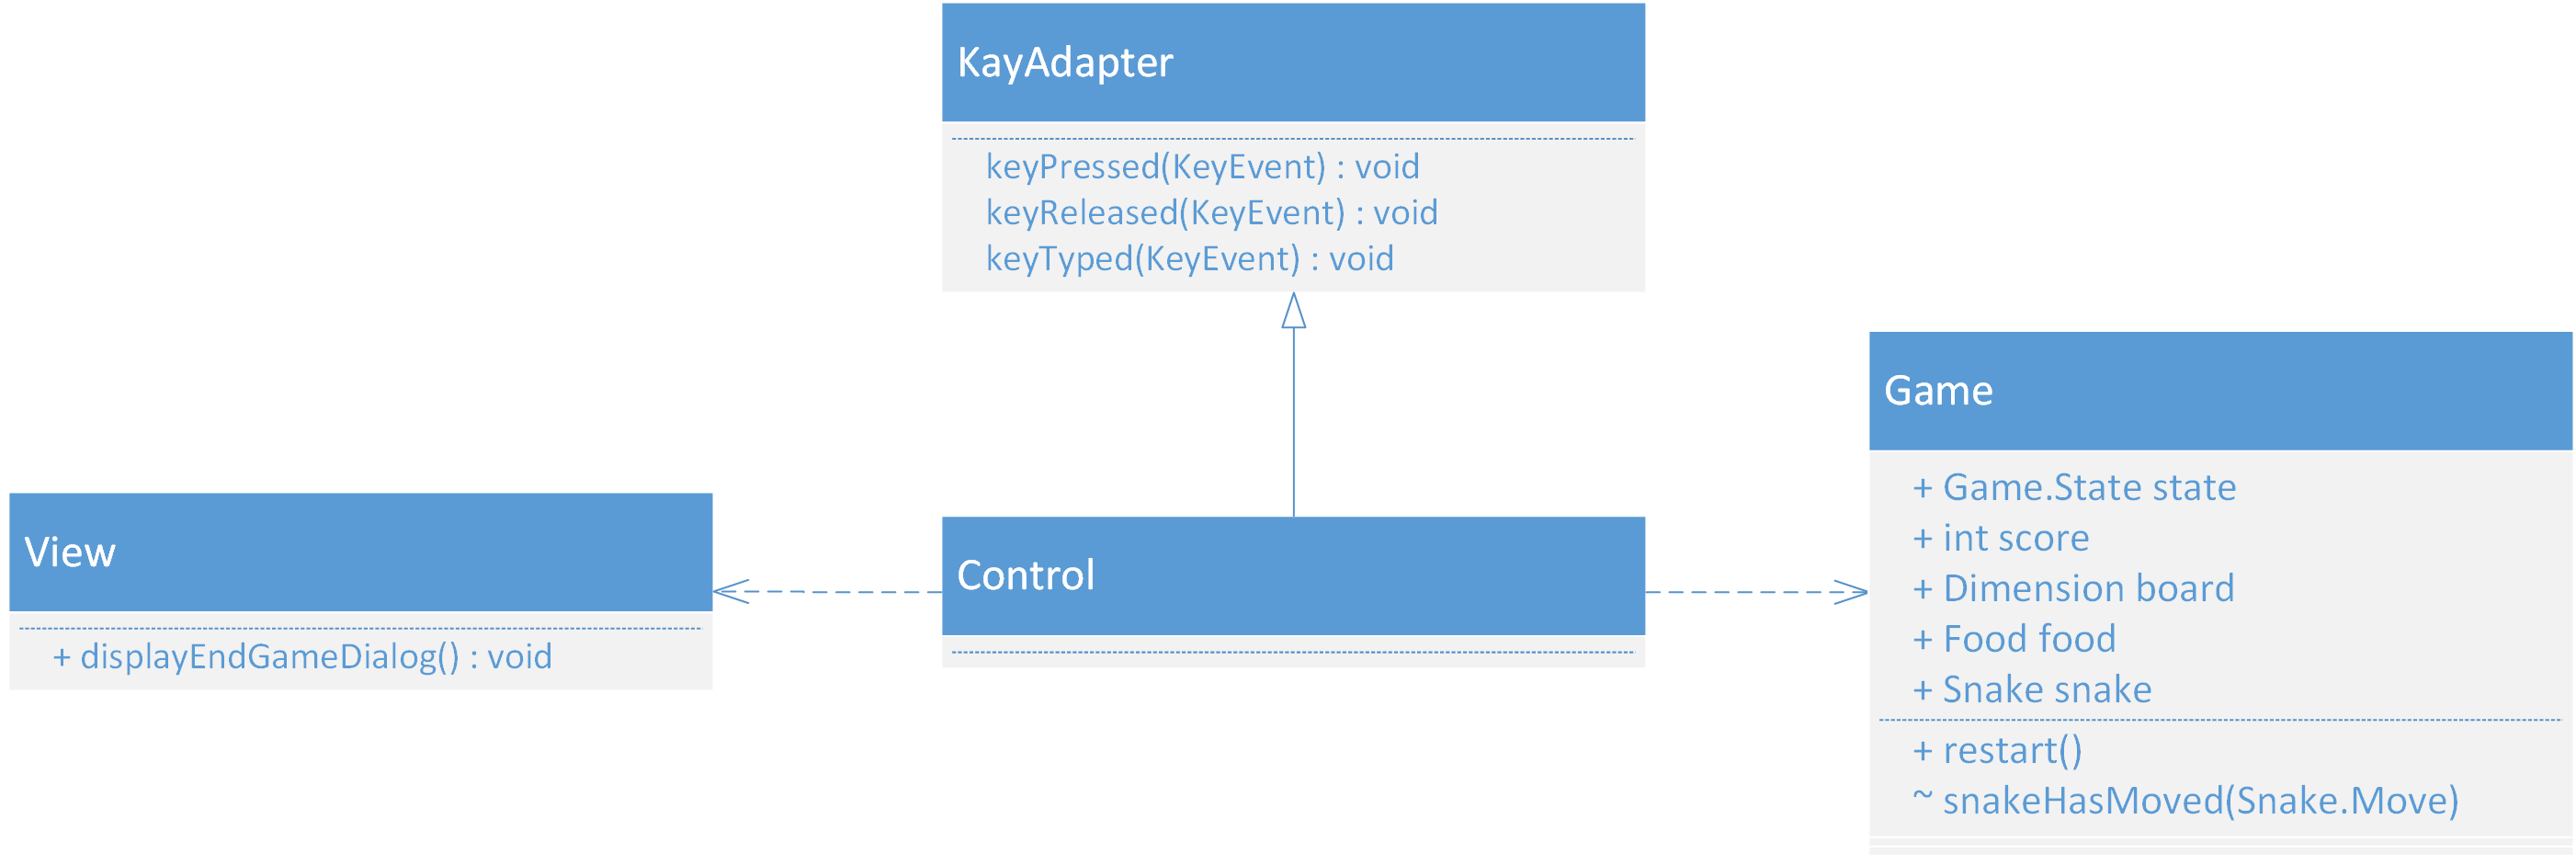
\includegraphics[width=1.0\textwidth]{grundlaeggende/control.png}
	\hspace{0.1\textwidth}
	\caption{\figlab{controlsimple}Oversigt over vores Control design.}
\end{figure}

For at starte spillet bruges klassen \textit{Driver}, som opretter et \textit{Game}-, \textit{View} og \textit{Control}-objekt.